\documentclass{standalone}
\usepackage{fontspec}
\setmainfont{Arial}
\usepackage{tikz}
\begin{document}

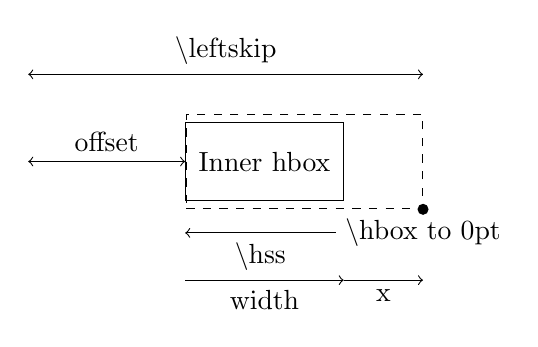
\begin{tikzpicture}
\coordinate (zero) at (0,0);

% The boxes
\node (innerbox) at (3,3) [draw,minimum width=2cm,minimum height=1cm] {Inner hbox};
\path (innerbox.east) +(-0.5,0) coordinate(outercenter);
\node (outerbox) at (outercenter) [draw,dashed,minimum width=3cm,minimum height=1.2cm]{};
\fill (outerbox.south east) circle(2pt) node(zptnode)[anchor=north]{\textbackslash hbox to 0pt};

'% leftskip, offset
\path (outerbox.north east) ++(0,0.5) coordinate(leftskipend);
\draw[<->] (zero |- leftskipend) -- (leftskipend) node[midway,anchor=south]{\textbackslash leftskip};
\draw[<->] (zero |- innerbox.west) -- (innerbox.west) node[midway,anchor=south]{offset};

% hbox to 0pt arrows
\draw[->] (zptnode.west) -- (innerbox.west |- zptnode.west) coordinate(hssleft) node[midway,anchor=north]{\textbackslash hss};
\path (hssleft) ++(0,-0.6) coordinate(widthleft);
\draw[->] (widthleft) -- (innerbox.east |- widthleft) node[midway,anchor=north]{width};
\draw[->] (innerbox.east |- widthleft) -- (outerbox.east |- widthleft) node[midway,anchor=north]{x};

\end{tikzpicture}

\end{document}
